\documentclass[tikz,border=5pt]{standalone}
\usepackage[T1]{fontenc}
\usepackage{lmodern,amsmath,amssymb}
\usetikzlibrary{arrows.meta,calc,positioning,fit,backgrounds,shapes.geometric,matrix,decorations.pathreplacing,patterns}
\definecolor{ink}{gray}{0.08}
\definecolor{wash}{gray}{0.965}
\definecolor{soft}{gray}{0.45}
\tikzset{box/.style={draw=ink,line width=.65pt,fill=white,align=center,inner sep=4pt,outer sep=0pt,font=\small},flow/.style={draw=ink,line width=.65pt,-{Latex[length=1.8mm,width=1.3mm]},rounded corners=2pt},annotation/.style={font=\scriptsize,text=soft,align=center},groupbox/.style={draw=soft,dashed,line width=.45pt,fill=wash}}
\begin{document}
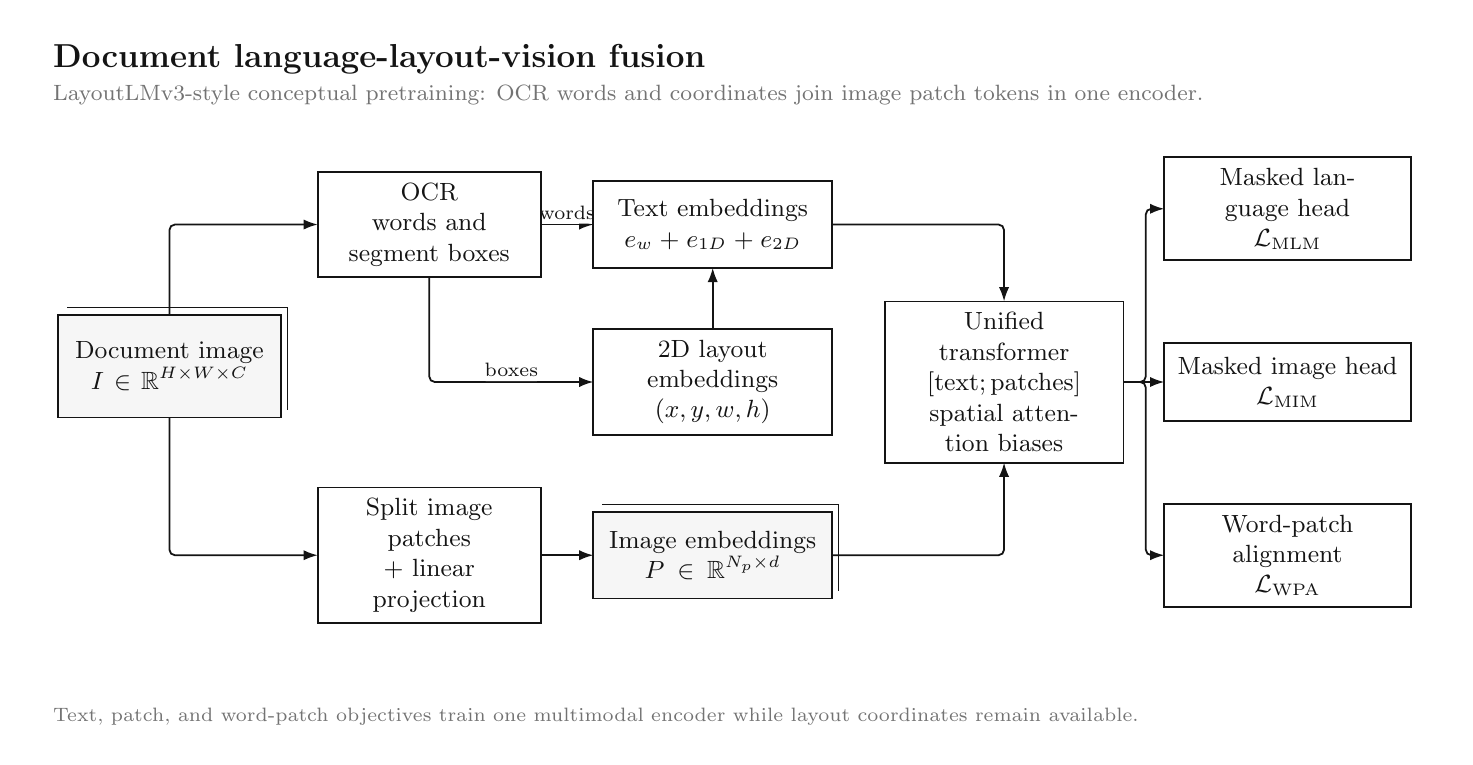
\begin{tikzpicture}[x=1cm,y=-1cm,font=\rmfamily,text=ink]

\path[use as bounding box] (0,0) rectangle (18,9);
\node[anchor=west,font=\large\bfseries] at (.2,.4) {Document language-layout-vision fusion};
\node[anchor=west,font=\footnotesize,text=soft] at (.2,.85) {LayoutLMv3-style conceptual pretraining: OCR words and coordinates join image patch tokens in one encoder.};
\begin{pgfonlayer}{background}
\end{pgfonlayer}
\node[box,fill=wash,minimum width=2.8cm,minimum height=1.3cm,text width=2.55cm] (page) at (1.8,4.3) {Document image\\$I\in\mathbb{R}^{H\times W\times C}$};
\draw[ink,line width=.4pt] (0.5000000000000001,3.55) -- (3.3000000000000003,3.55) -- (3.3000000000000003,4.8500000000000005);
\node[box,minimum width=2.8cm,minimum height=1.1cm,text width=2.55cm] (ocr) at (5.1,2.5) {OCR\\words and segment boxes};
\node[box,minimum width=2.8cm,minimum height=1.1cm,text width=2.55cm] (patch) at (5.1,6.7) {Split image patches\\+ linear projection};
\node[box,minimum width=3.0cm,minimum height=1.1cm,text width=2.75cm] (text) at (8.7,2.5) {Text embeddings\\$e_w+e_{1D}+e_{2D}$};
\node[box,minimum width=3.0cm,minimum height=1.1cm,text width=2.75cm] (layout) at (8.7,4.5) {2D layout embeddings\\$(x,y,w,h)$};
\node[box,fill=wash,minimum width=3.0cm,minimum height=1.1cm,text width=2.75cm] (image) at (8.7,6.7) {Image embeddings\\$P\in\mathbb{R}^{N_p\times d}$};
\draw[ink,line width=.4pt] (7.299999999999999,6.050000000000001) -- (10.299999999999999,6.050000000000001) -- (10.299999999999999,7.15);
\node[box,minimum width=3.0cm,minimum height=1.8cm,text width=2.75cm] (encoder) at (12.4,4.5) {Unified transformer\\$[\mathrm{text};\mathrm{patches}]$\\spatial attention biases};
\node[box,minimum width=3.1cm,minimum height=1.0cm,text width=2.85cm] (mlm) at (16.0,2.3) {Masked language head\\$\mathcal L_{\mathrm{MLM}}$};
\node[box,minimum width=3.1cm,minimum height=1.0cm,text width=2.85cm] (mim) at (16.0,4.5) {Masked image head\\$\mathcal L_{\mathrm{MIM}}$};
\node[box,minimum width=3.1cm,minimum height=1.0cm,text width=2.85cm] (wpa) at (16.0,6.7) {Word-patch alignment\\$\mathcal L_{\mathrm{WPA}}$};
\begin{pgfonlayer}{background}
\draw[flow] (page.north) -- (1.8,2.5) -- (ocr.west);
\draw[flow] (page.south) -- (1.8,6.7) -- (patch.west);
\draw[flow] (ocr.east) -- (text.west) node[midway,above,fill=white,inner sep=1.5pt,font=\scriptsize] {words};
\draw[flow] (ocr.south) -- (5.1,4.5) -- (layout.west) node[midway,above,fill=white,inner sep=1.5pt,font=\scriptsize] {boxes};
\draw[flow] (layout.north) -- (text.south);
\draw[flow] (patch.east) -- (image.west);
\draw[flow] (text.east) -- (12.4,2.5) -- (encoder.north);
\draw[flow] (image.east) -- (12.4,6.7) -- (encoder.south);
\draw[flow] (encoder.east) -- (14.2,4.5) -- (14.2,2.3) -- (mlm.west);
\draw[flow] (encoder.east) -- (mim.west);
\draw[flow] (encoder.east) -- (14.2,4.5) -- (14.2,6.7) -- (wpa.west);
\end{pgfonlayer}
\node[anchor=west,align=left,font=\scriptsize,text=soft,text width=17.6cm] at (.2,8.75) {Text, patch, and word-patch objectives train one multimodal encoder while layout coordinates remain available.};
\end{tikzpicture}
\end{document}
